\documentclass[border=10pt]{standalone}
\usepackage{pgfplots}
\usepgfplotslibrary{colormaps}
\begin{document}
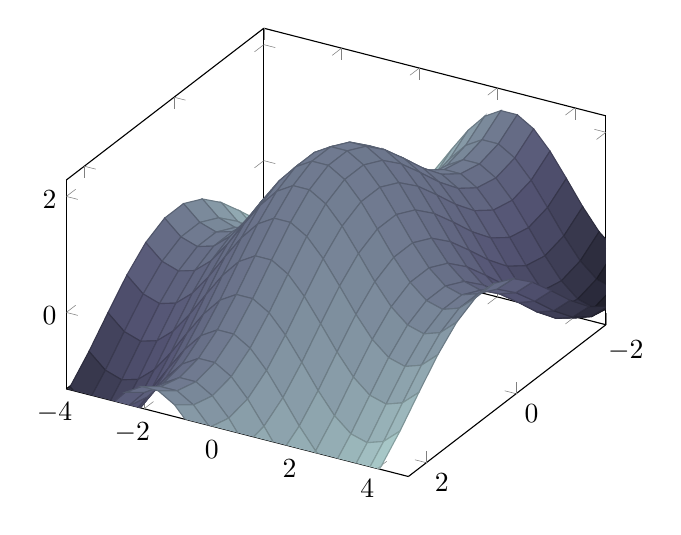
\begin{tikzpicture}
  \begin{axis}[
    view={120}{40},
   % grid=major,
    xmin=-2,xmax=2,
    ymin=-4,ymax=4,
    %zmin=-1,zmax=10,
    enlargelimits=upper,
    colormap/bone,
    trig format plots=rad,
  ]
  \addplot3 [ surf, domain=-4:4, domain y=-4:4,
              samples=20, samples y=20,
              variable=\u, variable y=\v,
              point meta=u*v ]
            ( {u}, {v}, {cos(u) + cos(v)} );
  \end{axis}
\end{tikzpicture}

\begin{tikzpicture}
  \begin{axis}
    \addplot3 (x, y, {x^2 + y^2});
    \addplot plot coordinates {
 (5, 8.312e-02,1)
 };
  \end{axis}

\end{tikzpicture}
\end{document}

%%% Local Variables:
%%% mode: latex
%%% TeX-master: t
%%% End:
